% Necoyoad Architecture Blueprint v11 — .htaccess Multi-Domain Routing + Widget Engine Preservation
\documentclass[11pt,a4paper]{article}
\usepackage[T1]{fontenc}
\usepackage[utf8]{inputenc}
\usepackage{lmodern}
\usepackage{microtype}
\usepackage{graphicx}
\usepackage{xcolor}
\usepackage{geometry}
\usepackage{amsmath}
\usepackage{amssymb}
\usepackage{tcolorbox}
\tcbuselibrary{skins,breakable,listings}
\usepackage{colortbl}
\usepackage{booktabs}
\usepackage{tabularx}
\usepackage{longtable}
\usepackage{array}
\usepackage{enumitem}
\usepackage{adjustbox}
\usepackage{caption}
\usepackage{fancyhdr}
\usepackage{titlesec}
\usepackage{pdflscape}
\usepackage{listings}
\usepackage{tikz}
\usetikzlibrary{arrows.meta,positioning,calc,shapes.geometric,fit,backgrounds,chains,decorations.pathreplacing,shapes.multipart}
\usepackage[colorlinks=true,linkcolor=blue!50!black,citecolor=blue!40!black,urlcolor=blue!60!black,bookmarks=true,bookmarksnumbered=true,unicode=true,pdftitle={Necoyoad - .htaccess Multi-Domain + Widget Engine Preservation (v11)},pdfauthor={Reverse-Engineered Architecture Report},pdfsubject={htaccess, Multi-Domain, Multi-Store, Widget Engine, Preservation Strategy},pdfkeywords={Necoyoad, OpenCart, PHP 8.1, htaccess, mod_rewrite, multi-domain, multi-store, widget engine, preservation, Laravel, Blade, Livewire}]{hyperref}
\geometry{a4paper, top=2.4cm, bottom=2.4cm, left=2.4cm, right=2.4cm}
\setlength{\headheight}{14pt}
\pagestyle{fancy}
\fancyhf{}
\fancyhead[L]{\small\itshape Necoyoad v11 --- .htaccess + Widget Engine Preservation}
\fancyfoot[C]{\small\thepage}
\renewcommand{\headrulewidth}{0.3pt}
\renewcommand{\footrulewidth}{0pt}
\titleformat{\section}{\Large\bfseries\color{black!85}}{\thesection}{0.6em}{}
\titleformat{\subsection}{\large\bfseries\color{black!80}}{\thesubsection}{0.6em}{}
\titleformat{\subsubsection}{\normalsize\bfseries\color{black!75}}{\thesubsubsection}{0.5em}{}
\widowpenalty=10000
\clubpenalty=10000
\emergencystretch=4em
\hbadness=10000
\hfuzz=2pt
\vfuzz=2pt
\sloppy
\definecolor{necoyoad-blue}{HTML}{1F4E79}
\definecolor{necoyoad-orange}{HTML}{B85C00}
\definecolor{necoyoad-green}{HTML}{2E6B33}
\definecolor{nodefill}{HTML}{F4F7FB}
\definecolor{nodefillalt}{HTML}{FBF4EE}
\definecolor{nodefillgreen}{HTML}{F2F8F2}
\definecolor{nodefillgray}{HTML}{F0F0F2}
\definecolor{phpline}{HTML}{F8F8F0}
\definecolor{phpcomment}{HTML}{8C8C8C}
\definecolor{phpkeyword}{HTML}{1F4E79}
\definecolor{phpstring}{HTML}{B85C00}
\lstdefinelanguage{necophp}{
  morekeywords={abstract,and,array,as,break,case,catch,class,clone,const,continue,declare,default,do,echo,else,elseif,empty,enddeclare,endfor,endforeach,endif,endswitch,endwhile,extends,final,finally,for,foreach,function,global,goto,if,implements,include,include_once,instanceof,insteadof,interface,namespace,new,or,print,private,protected,public,require,require_once,return,static,switch,throw,trait,try,use,var,while,xor,yield,true,false,null},
  sensitive=true,
  morecomment=[l]{//},
  morecomment=[s]{/*}{*/},
  morecomment=[l]{\#},
  morestring=[b]",
  morestring=[b]',
}
\lstset{
  language=necophp,
  basicstyle=\ttfamily\footnotesize,
  keywordstyle=\color{phpkeyword}\bfseries,
  commentstyle=\color{phpcomment}\itshape,
  stringstyle=\color{phpstring},
  backgroundcolor=\color{phpline},
  numbers=left,
  numberstyle=\tiny\color{phpcomment},
  numbersep=8pt,
  frame=single,
  rulecolor=\color{black!25},
  framerule=0.3pt,
  breaklines=true,
  breakatwhitespace=true,
  showstringspaces=false,
  captionpos=b,
  xleftmargin=14pt,
  xrightmargin=4pt,
  aboveskip=8pt,
  belowskip=8pt,
}
\newtcolorbox{keybox}[1][]{
  enhanced, breakable,
  colback=nodefill, colframe=necoyoad-blue!60,
  boxrule=0.4pt, arc=2pt, left=8pt, right=8pt, top=6pt, bottom=6pt,
  fonttitle=\bfseries\small, coltitle=white,
  title=#1
}
\captionsetup{justification=raggedright, singlelinecheck=false, font=small, labelfont=bf}

\begin{document}
\thispagestyle{empty}
\begin{center}
{\Large\bfseries Necoyoad --- .htaccess Multi-Domain Routing + Widget Engine Preservation (v11)}\\[0.4em]
{\small\itshape The Apache rewrite rules that power multi-domain multi-store,\\
and how to preserve the widget engine in a future framework}\\[1.2em]
\end{center}
\begin{abstract}
\noindent
This is the eleventh and final technical volume. It covers two topics the
user identified as critical: (1) the \texttt{.htaccess} rewrite rules that
integrate with the multi-domain multi-store feature, and (2) the widget
engine --- the platform's most valuable architectural asset --- and how to
preserve its full flexibility when migrating to a modern framework like
Laravel.

Part I dissects the three-layer \texttt{.htaccess} configuration (root
$\to$ \texttt{/web/} $\to$ \texttt{index.php}) that enables multi-domain
routing: the root \texttt{.htaccess} rewrites everything to
\texttt{/web/}, the \texttt{web/.htaccess} rewrites to
\texttt{index.php?\_route\_=}, and \texttt{index.php} itself detects the
store via URL path, GET parameter, or subdomain regex. Together, these
three layers implement a transparent multi-domain multi-store routing
system where each domain (or subdomain, or URL path prefix) maps to a
different store.

Part II is the widget engine preservation strategy. It identifies the
seven core abstractions that make the widget engine flexible
(\texttt{loadWidgets}, \texttt{NecoWidget}, the
\texttt{\{\%widget\_name\%\}} substitution, the
\texttt{module:settings} filter, the \texttt{Module} base class, the
\texttt{deps.php} manifest, and the per-entity/per-item composition), and
provides a concrete implementation plan for preserving each in a Laravel
or custom-framework rebuild. The goal: the same ``drop a widget into a
position, configure it in the admin, see it on the page'' developer
experience, with the same dynamic/manual/hybrid composition modes.
\end{abstract}
\vspace{0.6em}
\noindent\textbf{Keywords:} Necoyoad, OpenCart, PHP 8.1, .htaccess,
mod\_rewrite, multi-domain, multi-store, widget engine, preservation,
Laravel, Blade, Livewire, View Composers, dynamic components.
\newpage
\tableofcontents
\newpage

% ============================================================
\part{The .htaccess Multi-Domain Multi-Store Routing}\label{part:htaccess}
% ============================================================

\section{The Three-Layer Rewrite Architecture}\label{sec:three-layers}

Necoyoad uses three layers of URL rewriting to route requests to the
correct store:

\begin{enumerate}[leftmargin=1.6em,itemsep=2pt]
  \item \textbf{Root \texttt{.htaccess}} (253 lines) --- rewrites all
        requests to \texttt{/web/} (the web root). Also handles
        www-stripping and subdomain normalisation.
  \item \textbf{\texttt{web/.htaccess}} (611 lines) --- rewrites
        non-file, non-directory requests to
        \texttt{index.php?\_route\_=}. This is the SEO-URL entry point.
  \item \textbf{\texttt{web/index.php}} (85 lines) --- detects the
        store via three strategies (URL path, GET param, subdomain)
        and loads the matching \texttt{app/<store>/config.php}.
\end{enumerate}

\begin{figure}[htbp]
\centering
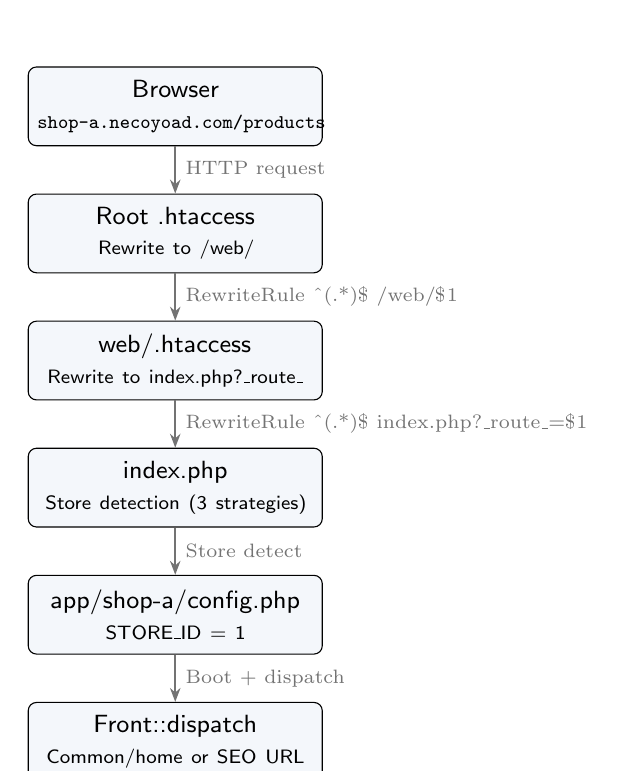
\begin{tikzpicture}[
  box/.style={draw, rounded corners=3pt, text width=3.5cm, minimum height=1.0cm, align=center, font=\small\sffamily, fill=nodefill},
  arr/.style={-{Stealth[length=5pt]}, thick, black!55}
]
  \node[box] (browser) {Browser\\\scriptsize \texttt{shop-a.necoyoad.com/products}};
  \node[box, below=0.6cm of browser] (root) {Root .htaccess\\\scriptsize Rewrite to /web/};
  \node[box, below=0.6cm of root] (web) {web/.htaccess\\\scriptsize Rewrite to index.php?\_route\_};
  \node[box, below=0.6cm of web] (index) {index.php\\\scriptsize Store detection (3 strategies)};
  \node[box, below=0.6cm of index] (config) {app/shop-a/config.php\\\scriptsize STORE\_ID = 1};
  \node[box, below=0.6cm of config] (dispatch) {Front::dispatch\\\scriptsize Common/home or SEO URL};

  \draw[arr] (browser) -- node[right, font=\scriptsize] {HTTP request} (root);
  \draw[arr] (root) -- node[right, font=\scriptsize] {RewriteRule \^{}(.*)\$ /web/\$1} (web);
  \draw[arr] (web) -- node[right, font=\scriptsize] {RewriteRule \^{}(.*)\$ index.php?\_route\_=\$1} (index);
  \draw[arr] (index) -- node[right, font=\scriptsize] {Store detect} (config);
  \draw[arr] (config) -- node[right, font=\scriptsize] {Boot + dispatch} (dispatch);
\end{tikzpicture}
\caption{The three-layer rewrite architecture. The root .htaccess
rewrites to /web/, the web/.htaccess rewrites to index.php, and
index.php detects the store and dispatches.}
\label{fig:three-layers}
\end{figure}

\section{The Root .htaccess}\label{sec:root-htaccess}

The root \texttt{.htaccess} (253 lines) serves two purposes:
\begin{enumerate}[leftmargin=1.6em,itemsep=2pt]
  \item \textbf{Rewrite to /web/}: all requests are internally
        redirected to the \texttt{/web/} subdirectory (where
        \texttt{index.php} lives).
  \item \textbf{Subdomain normalisation}: strips \texttt{www.} and
        normalises subdomains for the \texttt{necoyoad.com} domain.
\end{enumerate}

\begin{lstlisting}[caption={Root .htaccess --- the rewrite rules (abridged).},label={lst:root-htaccess}]
<IfModule mod_rewrite.c>
  Options +FollowSymlinks
  Options -Indexes
  RewriteEngine On
  RewriteBase /

  # Layer 1: Rewrite everything to /web/
  RewriteCond %{REQUEST_URI} !^/web/
  RewriteRule ^(.*)$ /web/$1 [L,QSA]

  # Layer 2: SEO URL rewrite (if not a real file/directory)
  RewriteCond %{REQUEST_FILENAME} !-f
  RewriteCond %{REQUEST_FILENAME} !-d
  RewriteRule ^(.*)\?*$ index.php?_route_=$1 [L,QSA]
</IfModule>

# www stripping
<IfModule mod_rewrite.c>
  RewriteCond %{HTTPS} !=on
  RewriteCond %{HTTP_HOST} ^www\.(.+)$ [NC]
  RewriteRule (.*) //%{HTTP_HOST}/$1 [R=301,L]
</IfModule>

# Subdomain normalisation (necoyoad.com only)
<IfModule mod_rewrite.c>
  RewriteCond %{HTTPS} !=on
  RewriteCond %{HTTP_HOST} !^necoyoad.com [NC]
  RewriteCond %{HTTP_HOST} ^([^.]+).necoyoad.com [NC]
  RewriteRule (.*)//%1.%{HTTP_HOST}/$1 [R=301,L]
</IfModule>

Options -MultiViews
ErrorDocument 404 /index.php?r=error/404
\end{lstlisting}

\subsection{The Rewrite-to-/web/ Rule}

\begin{lstlisting}[language={},basicstyle=\ttfamily\small,numbers=none,frame=none]
RewriteCond %{REQUEST_URI} !^/web/
RewriteRule ^(.*)$ /web/$1 [L,QSA]
\end{lstlisting}

This rule fires when the request URI does \emph{not} already start with
\texttt{/web/}. It prepends \texttt{/web/} to the URI. So a request to
\texttt{shop-a.necoyoad.com/products} becomes
\texttt{shop-a.necoyoad.com/web/products} (internally --- the browser
URL doesn't change). This lets the application live in a subdirectory
while appearing to serve from the root.

\subsection{The Subdomain Normalisation}

\begin{lstlisting}[language={},basicstyle=\ttfamily\small,numbers=none,frame=none]
RewriteCond %{HTTP_HOST} !^necoyoad.com [NC]
RewriteCond %{HTTP_HOST} ^([^.]+).necoyoad.com [NC]
RewriteRule (.*)//%1.%{HTTP_HOST}/$1 [R=301,L]
\end{lstlisting}

This rule fires when the host is a subdomain of
\texttt{necoyoad.com} (but not \texttt{necoyoad.com} itself). It
captures the subdomain label (\texttt{\%1}) and normalises the URL.
This is the Apache-level counterpart of the PHP subdomain regex in
\texttt{index.php} (v2, v5).

\subsection{Security Rules}

The root \texttt{.htaccess} also:
\begin{itemize}[leftmargin=1.6em,itemsep=2pt]
  \item Blocks access to dotfiles (\texttt{.git}, \texttt{.htaccess}
        itself) via \texttt{RewriteRule "(..|/)\textbackslash{}." - [F]}.
  \item Blocks access to sensitive file extensions
        (\texttt{.tpl}, \texttt{.bak}, \texttt{.config}, \texttt{.sql},
        \texttt{.ini}, \texttt{.log}, \texttt{.sh}, \texttt{.inc},
        \texttt{.swp}, \texttt{.dist}).
  \item Sets \texttt{session.cookie\_httponly true} for PHP sessions.
  \item Disables \texttt{MultiViews} (prevents Apache from
        content-negotiating, which would interfere with the rewrite
        rules).
\end{itemize}

\section{The web/.htaccess}\label{sec:web-htaccess}

The \texttt{web/.htaccess} (611 lines) is the main configuration file.
It handles:

\begin{itemize}[leftmargin=1.6em,itemsep=2pt]
  \item \textbf{SEO URL rewrite}: the core rule that sends everything
        to \texttt{index.php?\_route\_=}.
  \item \textbf{MIME types}: proper types for JS, fonts, SVG, video,
        audio.
  \item \textbf{Compression}: mod\_deflate for HTML, CSS, JS, JSON,
        XML, SVG, fonts.
  \item \textbf{Caching}: mod\_expires with per-type max-age (1 year
        for images/fonts, 1 week for CSS/JS, no cache for HTML).
  \item \textbf{CORS}: \texttt{Access-Control-Allow-Origin "*"} for
        fonts and images.
  \item \textbf{Security}: blocks dotfiles, blocks sensitive
        extensions, disables directory listing, custom 404/403
        error pages.
  \item \textbf{UTF-8}: \texttt{AddDefaultCharset utf-8} + per-type
        charset.
  \item \textbf{IE compatibility}: \texttt{X-UA-Compatible "IE=Edge"}.
  \item \texttt{ETag} and \texttt{Last-Modified} header management.
\end{itemize}

\subsection{The SEO URL Rewrite Rule}

\begin{lstlisting}[caption={web/.htaccess --- the SEO URL rewrite rule.},label={lst:web-rewrite}]
<IfModule mod_rewrite.c>
  Options +FollowSymlinks
  Options -Indexes
  RewriteEngine On
  RewriteBase /
  RewriteCond %{REQUEST_FILENAME} !-f
  RewriteCond %{REQUEST_FILENAME} !-d
  RewriteRule ^(.*)\?*$ index.php?_route_=$1 [L,QSA]
</IfModule>
\end{lstlisting}

This is the single most important rule in the entire \texttt{.htaccess}.
It says: if the request is not for a real file (\texttt{!-f}) and not
for a real directory (\texttt{!-d}), rewrite it to
\texttt{index.php?\_route\_=}. The \texttt{\_route\_} parameter carries
the URL path (e.g.\ \texttt{products/my-product}), which the PHP
\texttt{ControllerCommonSeoUrl} rewriter (v2) then resolves into a
controller route via the \texttt{url\_alias} table.

The \texttt{[L,QSA]} flags mean: Last (stop processing rules) and
Query String Append (preserve any existing GET parameters).

\section{The Multi-Domain Multi-Store Integration}\label{sec:multi-domain}

The \texttt{.htaccess} files don't directly implement multi-store
detection --- that's done in PHP (\texttt{index.php}). But they enable
it by:

\begin{enumerate}[leftmargin=1.6em,itemsep=2pt]
  \item \textbf{Transparent /web/ prefix}: the root \texttt{.htaccess}
        rewrites to \texttt{/web/} so the application doesn't need to
        know it's in a subdirectory. This means all stores share the
        same \texttt{.htaccess} rules regardless of their domain.
  \item \textbf{Subdomain passthrough}: the \texttt{.htaccess} does
        \emph{not} rewrite subdomains to specific directories. It
        passes the \texttt{HTTP\_HOST} header through to PHP, where
        \texttt{index.php} reads it and detects the store via the
        subdomain regex.
  \item \textbf{SEO URL passthrough}: the \texttt{\_route\_} parameter
        carries the full URL path. PHP's \texttt{ControllerCommonSeoUrl}
        then strips the store folder prefix (if present) and resolves
        the remaining path via \texttt{url\_alias}.
\end{enumerate}

\subsection{The Complete Multi-Domain Request Flow}

\begin{enumerate}[leftmargin=1.6em,itemsep=2pt]
  \item Browser requests \texttt{https://shop-a.necoyoad.com/products}.
  \item Root \texttt{.htaccess}: \texttt{REQUEST\_URI} does not start
        with \texttt{/web/}, so rewrite to
        \texttt{/web/products}. The \texttt{HTTP\_HOST} header
        (\texttt{shop-a.necoyoad.com}) is preserved.
  \item \texttt{web/.htaccess}: \texttt{/web/products} is not a real
        file or directory, so rewrite to
        \texttt{index.php?\_route\_=products}.
  \item \texttt{index.php}:
        \begin{enumerate}[itemsep=2pt]
          \item Strategy 1 (URL path): splits \texttt{products} by
                \texttt{/}, checks each segment against
                \texttt{store.folder}. No match.
          \item Strategy 2 (\texttt{?store\_id}): not set.
          \item Strategy 3 (subdomain regex): a \texttt{preg\_match}
                call captures the subdomain label from
                \texttt{shop-a.necoyoad.com}, yielding
                \texttt{\$matches[1] = 'shop-a'}.
          \item \texttt{file\_exists('app/shop-a/config.php')} $\to$ yes.
          \item Loads \texttt{app/shop-a/config.php} which sets
                \texttt{STORE\_ID = 1} and
                \texttt{DIR\_APPLICATION = 'app/shop-a/'}.
        \end{enumerate}
  \item \texttt{ControllerCommonSeoUrl}: resolves \texttt{products} via
        \texttt{url\_alias} $\to$ \texttt{store/product/all}.
  \item \texttt{Front::dispatch(new Action('store/product/all'))}.
\end{enumerate}

\subsection{Multi-Domain with Different Document Roots}

For domains that point to different document roots (not subdomains of
\texttt{necoyoad.com}), the \texttt{.htaccess} doesn't need modification
--- each domain's document root contains its own copy of the
\texttt{.htaccess} + \texttt{index.php}. The \texttt{index.php} store
detection still works via Strategy 1 (URL path folder match) or
Strategy 2 (\texttt{?store\_id} GET parameter).

% ============================================================
\part{The Widget Engine Preservation Strategy}\label{part:widget-engine}
% ============================================================

\section{Why the Widget Engine is the Most Valuable Asset}\label{sec:why-valuable}

The widget engine is the platform's crown jewel. It provides:

\begin{itemize}[leftmargin=1.6em,itemsep=2pt]
  \item \textbf{Drop-in composition}: an admin drags a widget into a
        position; the widget appears on the page. No code changes.
  \item \textbf{Per-entity overrides}: different widgets on each
        product, post, page, or category.
  \item \textbf{Per-item composition}: widgets on individual banner
        slides (v9).
  \item \textbf{Three composition modes}: dynamic (admin-configured),
        manual (hardcoded placeholders), hybrid.
  \item \textbf{Visual editing}: drag-and-drop via \texttt{nt-editable}
        attributes.
  \item \textbf{Asset management}: per-widget CSS/JS via
        \texttt{deps.php} manifest + route-aware loader.
  \item \textbf{Developer experience}: a new widget module is a
        controller + a template + an \texttt{install.php}. That's it.
\end{itemize}

No other part of the codebase provides this level of flexibility. The
admin CRUD, the marketing pipeline, the multi-store architecture ---
all are important, but the widget engine is what makes Necoyoad a
\emph{page builder}, not just an e-commerce platform.

\section{The Seven Core Abstractions}\label{sec:seven-abstractions}

To preserve the widget engine in a future framework, these seven
abstractions must be replicated:

\begin{table}[htbp]
\centering
\caption{The seven core widget engine abstractions.}\label{tab:seven}
\footnotesize\sloppy
\begin{tabularx}{\columnwidth}{>{\raggedright\arraybackslash}p{3.5cm}lX}
\toprule
\textbf{Abstraction} & \textbf{Current impl.} & \textbf{Role} \\
\midrule
1. \texttt{loadWidgets()} & \texttt{Controller} method & Queries the widget tree from the DB, merges widget routes into \texttt{\$children}. \\
2. \texttt{NecoWidget} & Helper class (785 lines) & The widget DAO: queries \texttt{property} EAV table, filters by device/lang/store/object. \\
3. \texttt{\{\%widget\_name\%\}} substitution & \texttt{Controller::fetch()} & Post-render string replacement of placeholder tokens with widget HTML. \\
4. \texttt{module:settings} filter & Hook on \texttt{Controller} & The seam where each widget module injects its data (banner items, product list, etc.). \\
5. \texttt{Module} base class & \texttt{system/classes/module.php} & Auto-loads \texttt{deps.php} assets for the widget's route. \\
6. \texttt{deps.php} manifest & Theme asset files & Declares which CSS/JS files apply to which routes. \\
7. Per-entity / per-item composition & Session \texttt{object\_type} + \texttt{NecoWidget::getWidgets()} & Widgets scoped to a specific product, post, page, category, or banner item. \\
\bottomrule
\end{tabularx}
\end{table}

\section{Preservation Strategy: Laravel Implementation}\label{sec:laravel-preservation}

\subsection{Abstraction 1: \texttt{loadWidgets()} $\to$ View Composer}

\begin{keybox}[Preserving loadWidgets as a View Composer]
In Laravel, \texttt{loadWidgets()} becomes a View Composer that runs
before every page render. The composer:

\begin{enumerate}[leftmargin=1.6em,itemsep=2pt]
  \item Reads the current route, store, language, device, and session
        \texttt{object\_type}.
  \item Queries the widget tree (via the WidgetService, see below).
  \item For each widget, instantiates its Blade component class and
        captures the rendered HTML.
  \item Publishes the widget HTML into the view as
        \texttt{\$widgets[\$position][\$widgetName]}.
  \item The Blade template iterates \texttt{\$widgets} and emits
        \texttt{<x-dynamic-component>} tags or raw HTML.
\end{enumerate}

The key insight: \texttt{loadWidgets()} is a \emph{view data
populator}, not a rendering mechanism. In Laravel, View Composers
serve exactly this role --- they populate view data before the view
renders. The widget tree structure (rows, columns, widgets) is
preserved as a nested array in the view data.
\end{keybox}

\subsection{Abstraction 2: NecoWidget $\to$ WidgetService}

\begin{keybox}[Preserving NecoWidget as a WidgetService]
The \texttt{NecoWidget} helper class (785 lines) becomes a
\texttt{WidgetService} Laravel service:

\begin{lstlisting}[language=PHP,basicstyle=\ttfamily\small,numbers=none,frame=none]
class WidgetService
{
    public function __construct(
        private WidgetRepository $widgets,
        private StoreContext $store,
        private LanguageContext $language,
    ) {}

    public function getTree(string $position, ?string $objectType = null, ?int $objectId = null): array
    {
        return $this->widgets->queryTree(
            storeId: $this->store->id(),
            languageId: $this->language->id(),
            position: $position,
            objectType: $objectType,
            objectId: $objectId,
        );
    }
}
\end{lstlisting}

The query changes from \texttt{LIKE} substring matching to a proper
JSON column query or a junction table. The device/auth/route/landing-page
filters are preserved as query conditions, not string-substring matches.
\end{keybox}

\subsection{Abstraction 3: \texttt{\{\%widget\_name\%\}} $\to$ Blade Slots}

\begin{keybox}[Preserving the placeholder substitution]
The \texttt{\{\%widget\_name\%\}} substitution becomes Blade's
\texttt{@stack} / \texttt{@push} or dynamic components.

\textbf{Option A: Dynamic Blade Components}

\begin{lstlisting}[language=PHP,basicstyle=\ttfamily\small,numbers=none,frame=none]
{{-- In the page template --}}
@foreach ($widgets['main'] as $row)
    @foreach ($row['columns'] as $column)
        @foreach ($column['widgets'] as $widget)
            <x-dynamic-component
                :component="$widget['component']"
                :settings="$widget['settings']"
            />
        @endforeach
    @endforeach
@endforeach
\end{lstlisting}

\textbf{Option B: Stack-based (for manual composition)}

\begin{lstlisting}[language=PHP,basicstyle=\ttfamily\small,numbers=none,frame=none]
{{-- In the page template (manual hardcoding) --}}
<div class="hero">
    @stack('hero_banner')
</div>
<div class="features">
    @stack('product_overview_1')
    @stack('product_overview_2')
</div>

{{-- In each widget's Blade component --}}
@push('hero_banner')
    <x-widgets.banner :banner="$banner" />
@endpush
\end{lstlisting}

Both options preserve the three composition modes:
\begin{itemize}[leftmargin=1.6em,itemsep=2pt]
  \item \textbf{Dynamic}: Option A --- the View Composer populates
        \texttt{\$widgets}, the template iterates.
  \item \textbf{Manual}: Option B --- the template uses
        \texttt{@stack}, the widget uses \texttt{@push}.
  \item \textbf{Hybrid}: both in the same template.
\end{itemize}
\end{keybox}

\subsection{Abstraction 4: \texttt{module:settings} Filter $\to$ Event Listener}

\begin{keybox}[Preserving the module:settings filter]
The \texttt{module:settings} filter (where each widget module injects
its data) becomes a Laravel Event/Listener:

\begin{lstlisting}[language=PHP,basicstyle=\ttfamily\small,numbers=none,frame=none]
// In the Banner widget's service provider
Event::listen(WidgetSettingsEvent::class, function ($event) {
    if ($event->widget->module === 'banner') {
        $banner = Banner::with('items.descriptions')
            ->findOrFail($event->settings['banner_id']);
        $event->data['banner'] = $banner;
        $event->template = "widgets.banner.{$banner->jquery_plugin}";
    }
});
\end{lstlisting}

The event fires for each widget before rendering. The listener
checks the module name, loads the widget's data, and sets the
template. This preserves the original's per-module injection pattern
while using Laravel's event system.
\end{keybox}

\subsection{Abstraction 5: Module Base Class $\to$ Blade Component Base}

\begin{keybox}[Preserving the Module base class]
The \texttt{Module} base class (which auto-loads \texttt{deps.php}
assets) becomes a base Blade Component:

\begin{lstlisting}[language=PHP,basicstyle=\ttfamily\small,numbers=none,frame=none]
abstract class WidgetComponent extends Component
{
    public function __construct(
        public array $settings,
        public ?object $widget = null,
    ) {
        // Auto-load this widget's assets (deps.php equivalent)
        app(AssetManifest::class)->loadForWidget(static::class);
    }

    // Subclasses override this to inject their data
    abstract public function data(): array;

    public function render()
    {
        return view($this->template, $this->data());
    }
}
\end{lstlisting}

Each widget module becomes a Blade Component that extends
\texttt{WidgetComponent}. The constructor auto-loads assets (the
\texttt{deps.php} equivalent). The \texttt{data()} method replaces
the \texttt{module:settings} filter --- each widget returns its own
data. The \texttt{render()} method uses the dynamic template
(per-entity or per-\texttt{jquery\_plugin}).
\end{keybox}

\subsection{Abstraction 6: deps.php Manifest $\to$ Vite Manifest + AssetManifest Service}

\begin{keybox}[Preserving the deps.php manifest]
The \texttt{deps.php} manifest (which declares which CSS/JS files
apply to which routes) becomes a Vite manifest + a Laravel
\texttt{AssetManifest} service:

\begin{lstlisting}[language=PHP,basicstyle=\ttfamily\small,numbers=none,frame=none]
class AssetManifest
{
    private array $loaded = [];

    public function loadForWidget(string $widgetClass): void
    {
        $widgetName = Str::kebab(class_basename($widgetClass));
        $manifest = $this->getManifest();

        foreach ($manifest as $asset => $routes) {
            if ($routes === '*' || in_array("module/{$widgetName}", $routes)) {
                if (!in_array($asset, $this->loaded)) {
                    $this->loaded[] = $asset;
                    // Push to Vite's tag resolver or Laravel Mix
                    app('asset')->enqueue($asset);
                }
            }
        }
    }
}
\end{lstlisting}

The manifest file changes from PHP to JSON or YAML, but the concept
is the same: declare which assets apply to which routes, and the
service loads matching assets for the current route.
\end{keybox}

\subsection{Abstraction 7: Per-Entity/Per-Item Composition $\to$ Query Scopes}

\begin{keybox}[Preserving per-entity and per-item widget composition]
The per-entity widget override (where product pages show
product-specific widgets) becomes a query scope on the
\texttt{WidgetRepository}:

\begin{lstlisting}[language=PHP,basicstyle=\ttfamily\small,numbers=none,frame=none]
class WidgetRepository
{
    public function queryTree(
        int $storeId,
        int $languageId,
        string $position,
        ?string $objectType = null,
        ?int $objectId = null,
    ): array {
        // Default tree (no object filter)
        $tree = WidgetRow::with('columns.widgets')
            ->where('store_id', $storeId)
            ->where('position', $position)
            ->where('landing_page', 'all')
            ->orWhere('landing_page', $this->currentRoute())
            ->orderBy('sort_order')
            ->get();

        // Per-object override (if objectType/objectId provided)
        if ($objectType && $objectId) {
            $objectWidgets = WidgetRow::with('columns.widgets')
                ->where('store_id', $storeId)
                ->where('position', $position)
                ->where('object_type', $objectType)
                ->where('object_id', $objectId)
                ->orderBy('sort_order')
                ->get();

            $tree = $tree->merge($objectWidgets);
        }

        return $tree->toArray();
    }
}
\end{lstlisting}

This preserves the two-query merge (default tree + per-object tree)
and the \texttt{only:} prefix (skip the default tree, load only the
per-object tree) by simply not running the first query when
\texttt{only} is set.
\end{keybox}

\section{The Developer Experience: Creating a New Widget}\label{sec:dev-experience}

\subsection{Current (Necoyoad)}

\begin{enumerate}[leftmargin=1.6em,itemsep=2pt]
  \item Create \texttt{app/admin/controller/module/<name>/widget.php}
        (admin config form).
  \item Create
        \texttt{app/shop/controller/module/<name>.php} (storefront
        controller, extends \texttt{Module}).
  \item Create
        \texttt{app/shop/view/theme/choroni/module/<name>.tpl}
        (storefront template).
  \item Create \texttt{install.php} + \texttt{uninstall.php}.
  \item Add CSS/JS to \texttt{web/assets/theme/<theme>/{css,js}/deps.php}.
  \item Done. The admin can now drag the widget into any position.
\end{enumerate}

\subsection{Future (Laravel)}

\begin{enumerate}[leftmargin=1.6em,itemsep=2pt]
  \item Create \texttt{app/Filament/Pages/Widgets/<Name>Settings.php}
        (admin config form, using Filament or Laravel Nova).
  \item Create
        \texttt{app/View/Components/Widgets/<Name>.php} (extends
        \texttt{WidgetComponent}).
  \item Create
        \texttt{resources/views/components/widgets/<name>.blade.php}
        (storefront template).
  \item Create a migration for the widget's default settings.
  \item Add CSS/JS to the Vite manifest.
  \item Done. The admin can now drag the widget into any position.
\end{enumerate}

The developer experience is essentially the same: a controller
(component), a template, a config form, and asset registration. The
key difference is that the Laravel version uses Blade components
instead of raw PHP templates, and Eloquent instead of raw SQL --- but
the \emph{concept} is identical.

\section{What Must NOT Change}\label{sec:must-not-change}

\begin{keybox}[Non-negotiable: the widget composition experience]
The following aspects of the widget engine \emph{must} be preserved
in any rebuild:

\begin{enumerate}[leftmargin=1.6em,itemsep=2pt]
  \item \textbf{The admin can compose pages without code}. A
        non-technical user drags widgets into positions, configures
        them via a form, and the page renders. This is the number-one feature.
  \item \textbf{Three composition modes}. Dynamic (admin-configured),
        manual (hardcoded placeholders in templates), and hybrid
        (both in the same template).
  \item \textbf{Per-entity overrides}. Different widgets on each
        product, post, page, category, or banner item.
  \item \textbf{The \texttt{module:settings} seam}. Each widget
        module has a single, well-defined injection point where it
        loads its data and selects its template.
  \item \textbf{The asset manifest}. CSS/JS files are declared in a
        manifest and auto-loaded for matching routes. The developer
        doesn't manually enqueue assets.
  \item \textbf{The visual editor hooks}. \texttt{nt-editable} (or
        equivalent) attributes on every widget wrapper, so a visual
        editor can identify and manipulate widgets.
  \item \textbf{Per-entity template override}. Each entity can use a
        different template, set via the admin, stored in EAV (or
        JSON column in Laravel).
\end{enumerate}
\end{keybox}

\section{The Widget Engine API Contract}\label{sec:api-contract}

To ensure the widget engine survives a framework migration, here is
the API contract that any future implementation must satisfy:

\begin{table}[htbp]
\centering
\caption{The widget engine API contract.}\label{tab:api-contract}
\footnotesize\sloppy
\begin{tabularx}{\columnwidth}{>{\raggedright\arraybackslash}p{4.0cm}X}
\toprule
\textbf{Capability} & \textbf{Contract} \\
\midrule
Query widgets by position & \texttt{getTree(position, objectType?, objectId?)} returns a nested array of rows, columns, widgets. \\
Register a widget module & A class that extends \texttt{WidgetComponent} + a Blade template + a settings form. \\
Inject widget data & A method (or event listener) that receives the widget settings and returns the data + template path. \\
Render a widget & The widget's Blade component renders its template with the injected data. \\
Compose dynamically & A View Composer populates \texttt{\$widgets[\$position]} before the page renders. \\
Compose manually & Templates can use \texttt{@stack} / \texttt{@push} or \texttt{<x-dynamic-component>} to hardcode widget positions. \\
Per-entity override & \texttt{getTree()} accepts \texttt{objectType} + \texttt{objectId} and merges per-object widgets into the default tree. \\
Per-item composition & Same as per-entity, with \texttt{objectType = 'banner\_item'} (or any other item type). \\
Asset loading & An \texttt{AssetManifest} service loads CSS/JS for the current route + widget modules. \\
Visual editor hooks & Every widget wrapper emits \texttt{data-widget}, \texttt{data-position}, \texttt{data-row}, \texttt{data-column} attributes. \\
Template override & Each entity can specify a template path (stored as a property/JSON column), resolved as: entity template $\to$ config default $\to$ hardcoded fallback. \\
\bottomrule
\end{tabularx}
\end{table}

% ============================================================
\section{Conclusion}\label{sec:conclusion}
% ============================================================

\subsection{The .htaccess is a Transparent Multi-Domain Enabler}

The \texttt{.htaccess} configuration (root + web) is a transparent
multi-domain enabler. It doesn't implement store detection --- it
passes the \texttt{HTTP\_HOST} and URL path through to PHP, where
\texttt{index.php} does the actual detection. The three-layer
architecture (root rewrite $\to$ web rewrite $\to$ PHP dispatch) allows
the application to live in a subdirectory while appearing to serve
from the root, and allows multiple domains to share the same codebase
with different stores.

\subsection{The Widget Engine is the Platform's Soul}

The widget engine is not just a feature --- it is the platform's soul.
It is what makes Necoyoad a page builder, not just an e-commerce
platform. The seven core abstractions
(\texttt{loadWidgets}, \texttt{NecoWidget}, the
\texttt{\{\%widget\_name\%\}} substitution, the
\texttt{module:settings} filter, the \texttt{Module} base class, the
\texttt{deps.php} manifest, and the per-entity/per-item composition)
together form a flexible composition system that allows
non-technical users to build complex pages by dragging widgets into
positions, and developers to create new widgets with minimal
boilerplate.

\subsection{The Preservation Strategy is Concrete}

The preservation strategy is not abstract --- each of the seven
abstractions has a concrete Laravel equivalent:
\begin{itemize}[leftmargin=1.6em,itemsep=2pt]
  \item \texttt{loadWidgets()} $\to$ View Composer
  \item \texttt{NecoWidget} $\to$ \texttt{WidgetService}
  \item \texttt{\{\%widget\_name\%\}} $\to$ Blade dynamic components /
        \texttt{@stack}
  \item \texttt{module:settings} $\to$ Event listener
  \item \texttt{Module} base $\to$ \texttt{WidgetComponent} base
  \item \texttt{deps.php} $\to$ Vite manifest + \texttt{AssetManifest}
  \item Per-entity composition $\to$ Query scopes on
        \texttt{WidgetRepository}
\end{itemize}

The developer experience --- ``create a controller, a template, a
config form, and register assets'' --- remains the same. The
framework changes; the concept doesn't.

\subsection{Final Word}

The Necoyoad widget engine is a genuinely innovative piece of
architecture. It anticipated by years the page-builder patterns that
WordPress's block editor, Drupal's Layout Builder, and Laravel's
Filament builder are only now popularising. Preserving it in a future
rebuild is not just about nostalgia --- it is about keeping the
platform's most valuable competitive advantage: the ability to compose
rich, interactive pages without writing code.

\end{document}
